\documentclass[11pt, a4paper, spanish]{article}
\usepackage{etex}

\usepackage[a4paper, margin=2.5cm, top=3.5cm, bottom=3.5cm]{geometry} % Define los márgenes
\usepackage{amsmath, amscd, amssymb, amsthm, latexsym, gensymb} % Paquetes matemáticos
\usepackage[spanish]{babel} % Traduce los paquetes a español
\usepackage[utf8]{inputenc} % Codificación UTF8
\usepackage{fancyhdr} % Encabezados y pies de página
  \pagestyle{fancyplain}
\usepackage{enumerate}
\usepackage{xspace}
\usepackage[page, toc]{appendix} % Apéndices
\usepackage[nottoc]{tocbibind} % Referencias en la TDC
\usepackage{scrextend} % Para usar addmargin
\usepackage{listings} % Código
  \lstdefinestyle{customcpp}{
    belowcaptionskip=1\baselineskip,
    breaklines=true,
    xleftmargin=3em,
    language=C++,
    basicstyle=\small\ttfamily
  }
\usepackage[onelanguage, spanish]{algorithm2e}
  % \NoCaptionOfAlgo
  \LinesNumbered\RestyleAlgo{ruled}\IncMargin{1em}\DontPrintSemicolon\SetArgSty{}\SetCommentSty{textsf}\SetFuncSty{textsf}
  \SetKwProg{For}{para}{ hacer}{fin}
  \SetKwProg{Fn}{función}{:}{fin}
\usepackage[pdftex]{graphicx} % Imágenes
\usepackage[usenames,dvipsnames]{color} % Autoexplicativo
% \usepackage{caption} % Captions sin números
% \usepackage{multirow} % Celdas multifila en tablas
\usepackage[thinlines]{easytable} % Tablas para diagramas de registros
\usepackage{tabu} % Tablas para diagramas de registros
\usepackage{caratula} % Carátula del DC

% Bibliografía
% \usepackage{biblatex}
% \addbibresource{referencias.bib}

% Comandos personalizados
\let\strong\textbf
\renewcommand{\appendixtocname}{Apéndices}
\renewcommand{\appendixpagename}{Apéndices}
\theoremstyle{plain}
  \newtheorem{prop}{Proposición}
  \newtheorem{lema}{Lema}
\theoremstyle{remark}
  \newtheorem{obs}{Observación}
\setlength{\parskip}{.3em}
\newcommand{\acr}[1]{\textsc{\lowercase{#1}}} % Acrónimos
\newcommand{\mat}[1]{\ensuremath{\mathbf{#1}}}
\newcommand{\img}[1]{\mat{#1}}
\newcommand{\comp}[1]{\ensuremath{\mathsf{#1}}}

\newenvironment{bitlimits}[2]{caca}{caca}

% Encabezado
\lhead{Organización del Computador II}
\rhead{Trabajo Práctico Nº 2}
% Pie de pagina
\renewcommand{\footrulewidth}{0.4pt}
% \lfoot{FCEN}
% \rfoot{UBA}

\begin{document}

% Datos de carátula
\materia{Organización del Computador II}
\titulo{Trabajo Práctico Nº 2}
\fecha{Segundo cuatrimestre de 2015}
\grupo{Grupo: Smelly Cat}

\integrante{Frizzo, Franco}{013/14}{francofrizzo@gmail.com}
\integrante{Martínez, Manuela}{160/14}{martinez.manuela.22@gmail.com}
\integrante{Rabinowicz, Lucía}{105/14}{lu.rabinowicz@gmail.com}

% Carátula
\maketitle
\newpage

% Índice
\tableofcontents
\clearpage

% Contenido
\section{Introducción}

  En el presente trabajo, aplicamos el modelo de programación vectorial \acr{SIMD} (\emph{Single Instruction, Multiple Data}) para la implementación de filtros para el procesamiento de imágenes. Más precisamente, llevamos a cabo la implementación de los siguientes dos filtros:
  \begin{itemize}
    \item \emph{Diferencia}, que recibe como entrada dos imágenes y devuelve como resultado otra imagen que indica dónde difieren las dos primeras.
    \item \emph{Blur gaussiano}, que suaviza la imagen reemplazando cada píxel por un promedio de los píxeles circundantes, ponderado según una función gaussiana.
  \end{itemize}

  La elaboración del trabajo se dividió en dos etapas. En primer lugar, implementamos ambos filtros tanto en lenguaje C como en lenguaje ensamblador para la arquitectura x86 de Intel. En este último caso, se utilizaron las instrucciones \acr{SSE} de dicha arquitectura, que aprovechan el ya mencionado modelo \acr{SIMD} para procesar datos en forma paralela.

  Una vez realizadas estas implementaciones, las sometimos a un proceso de comparación para extraer conclusiones acerca de su rendimiento. Con este fin, experimentamos con variaciones tanto en los datos de entrada como en detalles implementativos de los mismos algoritmos. De esta manera pudimos recopilar datos sobre el comportamiento de cada implementación, y contrastar estos resultados con diversas hipótesis previamente elaboradas.

% \clearpage
\section{Desarrollo}

  \subsection{Consideraciones generales}
    Las imagenes que utilizaremos como entrada y salida de los algoritmos a implementar serán matrices de píxeles. Cada uno de estos píxeles estará representado por cuatro enteros sin signo de 8 bits de profundidad (es decir, en el rango [0, 256)), que representarán, respectivamente, los valores de los colores azul (\textsf{b}), verde (\textsf{g}) y rojo (\textsf{r}), y la transparencia (\textsf{a}).

    Usaremos la notación $I_{x,y}$ para referirnos al píxel ubicado en la fila $x$ y la columna $y$ de la imagen $I$, y la notación $I_{x,y}^k$ para hacer referencia al valor de la componente $k$ de este píxel, donde $k \in \lbrace \mathsf{b, g, r, a} \rbrace$.
  
  \subsection{Diferencia de imágenes}
    Este filtro recibe dos imágenes como entrada y devuelve como salida una tercera imagen que muestra, en cada píxel, la diferencia entre los píxeles correspondientes de las imágenes de entrada, ignorando la componente \textsf{a}. Más especificamente, si $I_1$ e $I_2$ son las imágenes de entrada y $O$ es la imagen de salida, entonces:

    \[ O_{x,y}^k = \begin{cases}
      \displaystyle \max_{k \in \lbrace \mathsf{b, g, r} \rbrace} \left( \left\vert {I_1}_{x,y}^k - {I_2}_{x,y}^k \right\vert \right)
        & \text{si } k \in \lbrace \mathsf{b, g, r} \rbrace \\
      255
        & \text{si } k = \mathsf{a}
    \end{cases} \]

    \subsubsection{Implementación en lenguaje C}

    \subsubsection{Implementación en lenguaje ensamblador}
      Dado que los registros \texttt{XMM} son de 16 bytes, se los puede utilizar para procesar 4 píxeles de las imágenes en paralelo, reduciendo la cantidad de iteraciones del algoritmo y, particularmente, de accesos a memoria necesarios para completar el algoritmo.

      Nuestra implementación del filtro consiste principalmente de un ciclo que itera sobre la imagen. Al comienzo de cada ejecución, se copian 4 píxeles de $I_1$ al registro \texttt{XMM0}, y los correspondientes 4 píxeles de $I_2$ a \texttt{XMM1}.

      \raisebox{2.5mm}{\texttt{XMM0:} } \begin{TAB}(b,1cm,.8cm)[5pt]{|c|c|c|c|c|c|c|}{|c|}
        $A_4^{\mathsf{b}}$ &
        $A_4^{\mathsf{g}}$ &
        $A_4^{\mathsf{r}}$ &
        $A_4^{\mathsf{a}}$ &
        $A_3^{\mathsf{b}}$ &
        $\cdots$ &
        $A_1^{\mathsf{a}}$ \\
      \end{TAB}

      \raisebox{2.5mm}{\texttt{XMM1:} } \begin{TAB}(b,1cm,.8cm)[5pt]{|c|c|c|c|c|c|c|}{|c|}
        $B_4^{\mathsf{b}}$ &
        $B_4^{\mathsf{g}}$ &
        $B_4^{\mathsf{r}}$ &
        $B_4^{\mathsf{a}}$ &
        $B_3^{\mathsf{b}}$ &
        $\cdots$ &
        $B_1^{\mathsf{a}}$ \\
      \end{TAB}

      El paso siguiente es, para cada una de las componentes de estos píxeles, calcular el valor absoluto de la diferencia entre ambas imágenes. Para realizar esto, realizamos las dos restas, es decir, $\mathtt{XMM0} - \mathtt{XMM1}$ y $\mathtt{XMM1} - \mathtt{XMM0}$. En las posiciones donde el valor contenido en \texttt{XMM0} sea mayor que el de \texttt{XMM1}, será válido el resultado de la primera operación, mientras que en las demás posiciones deberemos quedarnos con el segundo resultado.

      Para seleccionar con cuál de los dos resultados quedarnos, utilizamos una máscara que obtenemos comparando los valores de \texttt{XMM0} y \texttt{XMM1}. Aquí nos encontramos con un problema, ya que debemos comparar enteros sin signo, y \acr{SSE} no brinda instrucciones para hacer esto. Es por eso que recurrimos a desempaquetar los números y considerarlos como enteros con signo de dos bytes, que sí podemos comparar.

      En primer lugar, usando la instrucción \texttt{PUNPCKLBW}, desempaquetamos las partes bajas de \texttt{XMM0} y \texttt{XMM1} en los registros \texttt{XMM2} y \texttt{XMM3}.

      \raisebox{2.5mm}{\texttt{XMM2:} } \begin{TAB}(b,1cm,.8cm)[5pt]{|c|c|c|c|c|c|c|c|c|}{|c|}
        0 &
        $A_2^{\mathsf{b}}$ &
        0 &
        $A_2^{\mathsf{g}}$ &
        0 &
        $A_2^{\mathsf{r}}$ &
        $\cdots$ &
        0 &
        $A_1^{\mathsf{a}}$ \\
      \end{TAB}

      \raisebox{2.5mm}{\texttt{XMM3:} } \begin{TAB}(b,1cm,.8cm)[5pt]{|c|c|c|c|c|c|c|c|c|}{|c|}
        0 &
        $B_2^{\mathsf{b}}$ &
        0 &
        $B_2^{\mathsf{g}}$ &
        0 &
        $B_2^{\mathsf{r}}$ &
        $\cdots$ &
        0 &
        $B_1^{\mathsf{a}}$ \\
      \end{TAB}


      Luego los comparamos mediante la instrucción \texttt{PCMPGTW}, almacenando la máscara resultante en \texttt{XMM2}. A continuación hacemos lo mismo con las partes altas, usando la instrucción \texttt{PUNPCKHBW} para desempaquetar y guardando el resultado en \texttt{XMM3}. Por último, la instrucción \texttt{PACKSSWB XMM2, XMM3} nos permite obtener en \texttt{XMM2} la máscara que buscábamos, ya que transforma los valores de 2 a 1 byte usando saturación.

  \subsection{Blur gaussiano}
    Este filtro recibe una imagen como entrada y devuelve como salida el resultado de aplicarle una convolución\footnote{Dadas dos funciones $f$ y $g$, una \emph{convolución} $f * g$ es una operación que las transforma en una tercera función: $(f * g)(t) = \int_{-\infty}^{+\infty} f(\tau) g(t - \tau) \,d\tau$ en el caso continuo, $(f * g)_n = \sum_{k=-\infty}^{+\infty} f_k g_{n-k}$ ($n, k \in \mathbb{Z}$) en el caso discreto.} con una función gaussiana, que dependerá de un parámetro $\sigma$ que podrá ser modificado. Dada la naturaleza del problema, trabajaremos con una convolución discreta en dos dimensiones, y como nuestro poder de cómputo es limitado, procesaremos solo una vecindad acotada de cada píxel, cuyo radio quedará determinado por un parámetro configurable $r$. En definitiva, el resultado del filtro será

    \[ O_{x,y}^k = \begin{cases}
      \displaystyle \sum_{i=-r}^r \sum_{j=-r}^r O_{x+i,y+j}^k K_{r-i,r-j}
        & \text{si } k \in \lbrace \mathsf{b, g, r} \rbrace \\
      255
        & \text{si } k = \mathsf{a}
    \end{cases} \]

    donde $K$ es la matriz o \emph{kernel} de la convolución, con

    \[ K_{i,j} = \frac{1}{2 \pi \sigma^2} e^{- \frac{(r-i)^2 + (r-j)^2}{2 \sigma^2}} \qquad \text{para todo } 0 \leq i,j \leq 2r \]

    \subsubsection{Implementación en lenguaje C}

    \subsubsection{Implementación en lenguaje ensamblador}

\section{Experimentación}
	Todos los experimentos se repitieron 20 veces. Para reproducirlos se debe ejecutar exp/exp.sh -n 20  

	\subsection{Experimento 1}
		En el primer experimento se genera una serie de imágenes de diferentes tamaños, tomando una imagen grande y disminuyendo progresivamente sus dimensiones.
		Luego, se ejecuta el filtro \emph{blur} con cada una de las imágenes generadas y se compara el tiempo de ejecución de las implementaciones en C y lenguaje ensamblador.
		Esto se repite para el filtro \emph{diff}, con la diferencia de que para cada tamaño de imagen se genera 
		un par de imágenes con ciertas diferencias entre ellas, para poder verificar el buen funcionamiento del mismo.

		\subsubsection*{Hipótesis} 
			Se espera observar que la implementación en lenguaje ensamblador de ambos filtros sea más eficiente, independientemente del tamaño de la imagen. Esto se debe a que hacen uso del modelo \acr{SIMD}, con todas las ventajas ya mencionadas que esto tiene sobre el rendimiento del código, a diferencia de las implementaciones de los algoritmos en C, que procesan cada píxel de manera independiente. Esto último puede inferirse no solo de la estructura propia del código, cuyos ciclos iteran sobre un único píxel a la vez, sino también de la ausencia de instrucciones \acr{SEE} para procesamiento de valores empaquetados que se observa al desensamblar los objetos obtenidos a partir de este código.

		\subsubsection*{Valores utilizados como parámetros} 		
			En este experimento el ancho de las imágenes utilizadas como parámetro se encuentran en un rango entre 24 y 1800 píxeles.Además, para el filtro Blur se utilizó $Radio = 15$ y $Sigma = 5$.

		\subsubsection*{Resultados}
		   	{\centering \begin{tabular}{c}
		      {\small Filtro Diferencia} \\
		      \includegraphics[width=12cm]{../exp/graficos/exp1-diff-c_vs_asm.png} \\
		    \end{tabular}}

		    {\centering \begin{tabular}{c}
		      {\small Filtro Diferencia - Tiempo de ejecución normalizado por píxel} \\
		      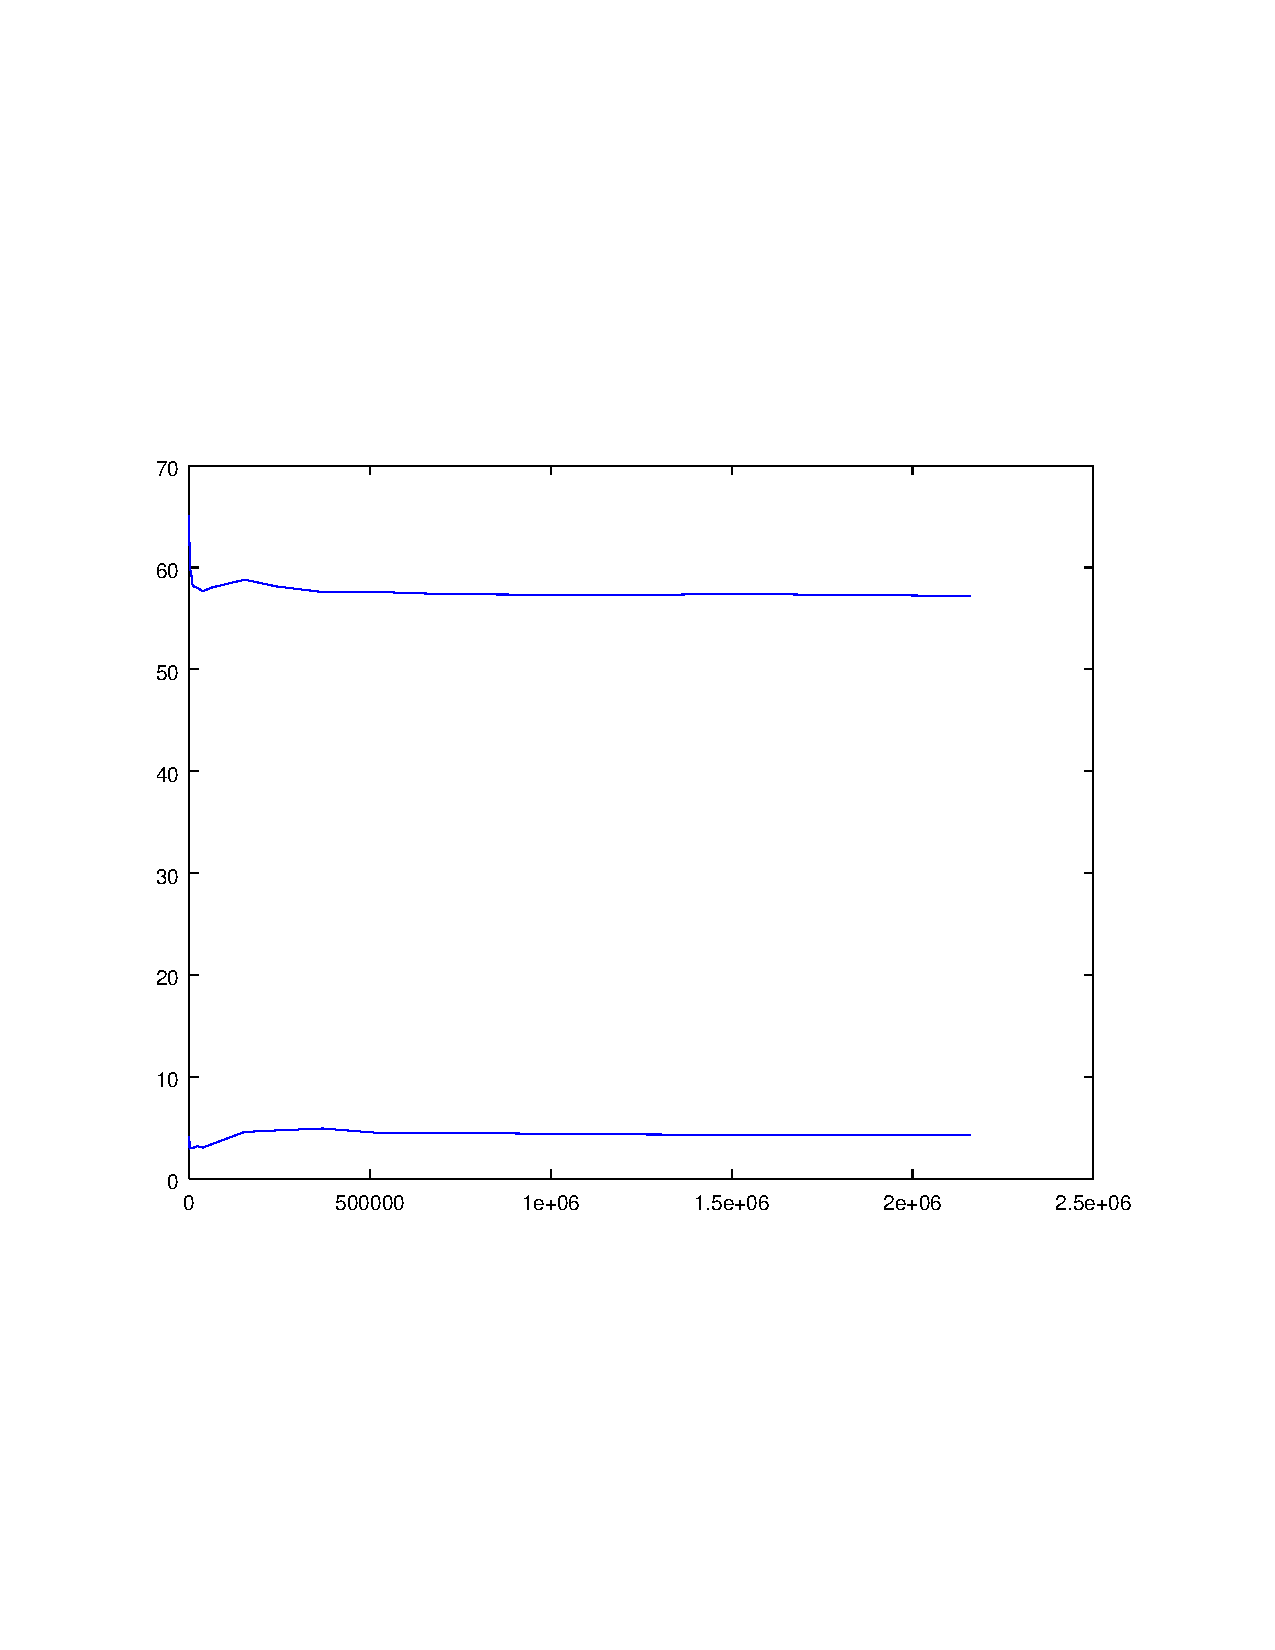
\includegraphics[width=12cm]{../exp/graficos/exp1-diff-tiempo_por_pixel.png} \\
		    \end{tabular}}

			{\centering \begin{tabular}{c}
		      {\small Filtro Blur} \\
		      \includegraphics[width=12cm]{../exp/graficos/exp1-blur-c_vs_asm.png} \\
		    \end{tabular}}

		   	{\centering \begin{tabular}{c}
		      {\small Filtro Blur - Tiempo de ejecución normalizado por píxel} \\
		      \includegraphics[width=12cm]{../exp/graficos/exp1-blur-tiempo_por_pixel.png} \\
		    \end{tabular}}

		\subsubsection*{Conclusiones y observaciones} 
			Como se observa en los resultados, se pudo confirmar la hipótesis planteada: la implementación en lenguaje ensamblador resultó más rápida que la implementación en C para todos los tamaños de imagen.
			En \emph{blur}, cuando llamamos a la función con un valor de $r$ mayor a la mitad de la altura o a la mitad del ancho de la imagen, no se producen cambios. Dado que en el experimento el valor de $r$ se mantiene constante, las dos imágenes más pequeñas no se ven afectadas por el filtro, lo cual se ve reflejado en los resultados, ya que para estas dos imágenes el tiempo de ejecución es notablemente menor.

	\subsection{Experimento 2}
		El objetivo de este experimento es observar como se ve afectada la eficiencia del algoritmo \emph{blur}, en ambas implementaciones, para diferentes valores del parámetro $r$ manteniendo constante la imagen de entrada.

		\subsubsection*{Hipótesis} 
			Se conjetura que, a medida que el valor del radio $r$ se incrementa, el tiempo de ejecución en las dos implementaciones aumentará, y que lo hará de manera cuadrática con respecto al incremento en $r$. Esto se debe a que la complejidad temporal de cada ejecución del ciclo principal del algoritmo depende del tamaño de la matriz de convolución, que es $(2 \times \mathtt{radio} + 1) \times (2 \times \mathtt{radio} + 1) \times 4$, es decir, es cuadrático en el valor de $r$.

		\subsubsection*{Valores utilizados como parámetros} 
		La dimensión de la imagen utilizada es 400 filas y 600 columnas. El valor del sigma es 5 y los radios toman valores entre 1 y 40.

		\subsubsection*{Resultados}

			{\centering \begin{tabular}{c}
	      		{\small Filtro Blur - Tiempo de ejecución según radio} \\
	      		\includegraphics[width=12cm]{../exp/graficos/exp2-tiempo_segun_radio.png} \\
	    	\end{tabular}}

		\subsubsection{Conclusiones y observaciones}
			Se puede observar en los gráficos que a medida que los $r$ aumenta, también lo hace el tiempo de ejecución. En este sentido, se pudo confirmar la hipótesis. Sin embargo, si se dividen los valores del tiempo de ejecución por su correspondiente $r^2$, se comprueba que la relación no es lineal; es decir, el tiempo de ejecución no varía cuadráticamente con el valor de $r$.


	\subsection{Experimento 3}
		Este experimento es similar al anterior, también se realiza sobre las dos implementaciones del filtro \emph{blur} y se considera siempre la misma imagen. En este caso el radio se mantiene constante pero el valor del sigma se modifica. También se va a utilizar el resultado normalizado, para poder estudiar el tiempo de procesamiento por píxel. 

			\subsubsection*{Hipótesis} 
				Debido a que el valor del sigma es utilizado solamente para realizar un cálculo por cada posición de la matriz de convolución, suponemos que modificar este valor no alterará el tiempo de ejecución.

			\subsubsection*{Valores utilizados como parámetros} 
			La dimensión de la imagen utilizada es 400 filas y 600 columnas. El valor del radio es 10 y sigma toma valores entre 0.5 y 50.

			\subsubsection*{Resultados}

			{\centering \begin{tabular}{c}
	      		{\small Filtro Blur - Tiempo de ejecución según sigma} \\
	      			\includegraphics[width=12cm]{../exp/graficos/exp3-tiempo_segun_sigma.png} \\
	    		\end{tabular}}

			\subsubsection*{Conclusiones y observaciones}
				Como dijimos en la hipótesis, la variación del sigma no afecta el tiempo de ejecución del algoritmo, tanto en lenguaje ensamblador como en C. Para valores de sigma menores que 1 podemos observar que el tiempo de ejecución es mayor.

				Esto se debe a que los valores serán muy grandes y el tiempo de ejecución de una cuenta aritmética deja e ser despreciable. 

	\subsection{Experimento 4}
		Otras de las pruebas consiste en comparar los tiempos de ejecución de diferentes implementaciones de los filtros en lenguaje ensamblador. Nos interesa medir el peso que tienen en el tiempo de ejecución los llamados a funciones auxiliares. Para esto, queremos comparar el rendimiento de una implementación que utiliza llamados a estas funciones, con el de otra que tiene todas las instrucciones necesarias en el mismo bloque de código (sin utilizar esas funciones auxiliares). 
		
		Este experimento se realiza una determinada cantidad de veces con distintos tamaños de imagen.

			\subsubsection*{Hipótesis} 
				Creemos que la versión del código implementada en lenguaje ensamblador que no realiza llamados a funciones va a tener un mejor rendimiento, ya que se evita el overhead que producen estos llamados.
		
			\subsubsection*{Valores utilizados como parámetros} 
				En este experimento el ancho de las imágenes utilizadas como parámetro se encuentran en un rango entre 24 y 1800 píxeles.Además, para el filtro Blur se utilizó $Radio = 15$ y $Sigma = 5$.


			\subsubsection*{Resultados}
				{\centering \begin{tabular}{c}
		      		{\small Filtro Diferencia} \\
		      		\includegraphics[width=12cm]{../exp/graficos/exp4-diff-c_vs_c2.png} \\
		    	\end{tabular}}

				{\centering \begin{tabular}{c}
		      		{\small Filtro Blur} \\
		      		\includegraphics[width=12cm]{../exp/graficos/exp4-blur-asm_vs_asm2.png} \\
		    	\end{tabular}}

			\subsubsection*{Conclusiones y observaciones}		

				Como muestran los gráficos de la implementación en C, los algoritmos que hacen llamados a otras funciones tienen un mayor tiempo de ejecución que las que no los hacen. Esto se debe a que cada vez que se hace un llamado a función, en necesario modificar la pila, manteniéndola alineada y guardando los registros que se deben preservar según la convención C y fueron utilizados a lo largo de la función.

				En lenguaje ensamblador, cuando implementamos el algoritmo sin el llamado a la función auxiliar, sigue siendo necesario acceder a la pila ya que hay que reutilizar registros que se tienen que mantener para la convención C. Por esto, seguimos haciendo accesos a memoria. Una vez que la accedemos es muy posible que en la cache se encuentren los siguientes accesos a realizar. Entonces la diferencia entre accederla unas pocas veces o mas es muy similar, ya que el acceso a memoria cache no es muy caro.

				Escribir un código en donde no realizamos llamadas a funciones auxiliares es mas difícil de mantener y además queda mas legible.

\clearpage

% Apéndices
% \input{apendices}
\clearpage

% Referencias
% \printbibliography[heading=bibintoc]

\end{document}
